% Chapter Template

\chapter{Results - Rubik's Cube} % Main chapter title

\label{sec:ResRubiks} % Change X to a consecutive number; for referencing this chapter elsewhere, use \ref{ChapterX}

%----------------------------------------------------------------------------------------
%	SECTION 1
%----------------------------------------------------------------------------------------

In this second results section, I discuss my experiments on the Rubik's cube. I have run reasonably comprehensive experiments on the 2x2x2, throwing 6 of my solvers at the problem. As mentioned in \ref{sec:Puzzles}, the 2x2x2 \textbf{RC}, in spite of its deceivingly simple physical appearance, is actually not that much easier to solve. For instance, it takes me usually just under 1 minute, whereras the 3x3x3 takes me only double that time, just under 2 minutes. I am obviously a beginner in Rubik's cube handsolving, but my personal ratio of time-to-solve and perceived difficulty is in line with that of experienced speedcubers who might take and average of, say, 2-3 seconds for the 2x2x2 and 10 seconds for the 3x3x3.
\\
Computing wise, the 2x2x2 was of decent size for my purpose, with its 88 million configurations, so in particular it 
\\
\\
Let me start with a table summarizing which solvers I have attempted to run on the 2 dimensions I have looked at:

\begin{center}
\begin{tabular}{l*{5}{c}r}
\hline
\textbf{solver}      & & \textbf{Rubik's} & \textbf{2x2x2} & \textbf{3x3x3} \\
\hline
BFS   &   &        &  x  &  x  \\
\hline
Kociemba   &   &      &  x  &  x  \\
\hline
A$^{*}$[Kociemba]  &   &  &  x  &  x  \\
\hline
A$^{*}$[DL[A$^{*}$[Kociemba]]]  &   &  &  x  &  x  \\
\hline
A$^{*}$[DRL]  &   &  &  x  &  \\
\hline
A$^{*}$[DQL]  &   &  &  x  &  \\
\hline
%MCTS[DQL][c=0]  &   &  & x &  \\
%\hline
%MCTS[DQL][c=69]  &   & & x &  \\
%\hline
\end{tabular}
\end{center}








\Section{2x2x2}
All the following experiments on the 2x2x2 \textbf{RC} have been run using my Solver's \textit{performance\_test} (see \ref{sec:codesolvers}): for each level of difficulty, the test present the solvers with the same 100 random configurations (for fairness and to increase the significance of the results). The levels of difficulty (number of scrambles from goal) used here go from 2 to 20 in step of 2. The tests were also run with perfect shuffling (difficulty = $\infty$ on the graphs), corresponding to taking scrambling to $\infty$ as explained in \ref{Theory:222RCSSS}).

\Subsection{BFS}
BFS is the only one for which I used a step of 1 on the difficuly and stopped at 5 as it was clear it would not go any further. Given that the run time and expanded nodes are clearly going to increase linearly, and give where difficulty of 5 took this solver already, there was no point going any further!

\Subsection{Kociemba, A$^{*}$[Kociemba], A$^{*}$[DL[A$^{*}$[Kociemba]]]}
Next, let me discuss Kociemba (\ref{}) and associated experiments. We obviously expect Kociemba to be by far the fastest solver since it is handcrafted with much specific knowledge about the Rubik's cube.






\Subsection{Deep reinforcement learner}
\label{sec:S33DRL}
Next I have run the DeepReinforcementLearner with the following main parameters:
\begin{itemize}
\item Update the target network every 1,000 epochs (\textit{update\_target\_network\_frequency=1000}) or when the MSE falls below 10 basis points of the maximum target cost-to-go (\textit{update\_target\_network\_threshold=1e-3})
\item Run for a maximum of 11,000 epochs (\textit{nb\_epochs=11000}) or when the maximum target so far has not been increasing by more than 1\% in the last 5,500 epochs (\textit{max\_target\_uptick=1e-2} and \textit{max\_target\_not\_increasing\_epochs\_pct=0.5})
\item At every update of the target network (\textit{training\_data\_every\_epoch=False}), generate 100 sequences of puzzles (\textit{nb\_sequences=100}), each comprised of a 50-scramble puzzle back to goal state, with all intermediary puzzles along the path (\textit{nb\_shuffles=50}).
\item Use a fully connected network (\textit{network\_type=fully\_connected\_net}) with three hidden layers of size 600, 300, 100 (\textit{layers\_description=(600,300,100)}) and use torch.optim.RMSProp as optimiser (\textit{optimiser=rms\_prop}) with an exponential scheduler (\textit{scheduler=exponential\_scheduler}) with gamma 0.999 (\textit{gamma\_scheduler=0.9999}).
\end{itemize}
Below I show some of the DeepReinforcementLearner's quantities tracked over the epochs (see \ref{fig:33SPDeepReinforcementLearning}). I have shown only the following quantities:
\begin{itemize}
\item learning rate, which decreases due to the scheduler, but gets reset at each network update.
\item max target. One interesting dynamic during learning is that due to the way targets are constructed using value-iteration update, and starting from an all 0 network, the max target only increases by about 1 at best at every network update. That is, the first network only learns how to differentiate goal from non-goal, then the second one learns how to differentiate goals, cost 1 and cost 2+ in some sense. This is why I have introduced the first set of parameters discussed just above. The first one makes sure we do not waste time initially training the left-hand-side network when training is easy (as consist of just goal versus not goal). The second ones make sure that we stop training altogether when the max target does not grow anymore. This is because we do not know a-priori what the God number of a given puzzle/dimension is, but let's assume for the sake of the argument that it is 15. Then that means that after 15 updates of the target network we might not really get so much benefit by keeping training and value-iterating.
\item the MSE loss
\item the MSE loss divided by the max target. The exit criterion \textit{update\_target\_network\_threshold} is based on that quantity, since a loss of e.g. 0.01 means little if the we do not compare it to the possible range that the cost-to-go can take.
\item The percentage of all the possible puzzles of that dimension \textit{seen} by the DeepReinforcementLearner. This is an interesting quantity, as it tells us later on when testing out of sample and comparing with other solvers, how well the solvers are able to generalise. In this case (3x3) we can see that the DeepReinforcementLearner quickly has seen a very large percentage of all puzzles. That being said, it is good to keep in mind that \textit{seen} does not mean really much here, since the learning is unsupervised. This is quite in contrast to the DeepLearner, for which puzzles seen come along with the cost-to-go computed by a \textit{teacher}, usually an optimal or at least efficient solver.
\end{itemize}


\begin{figure}[H]
\centering
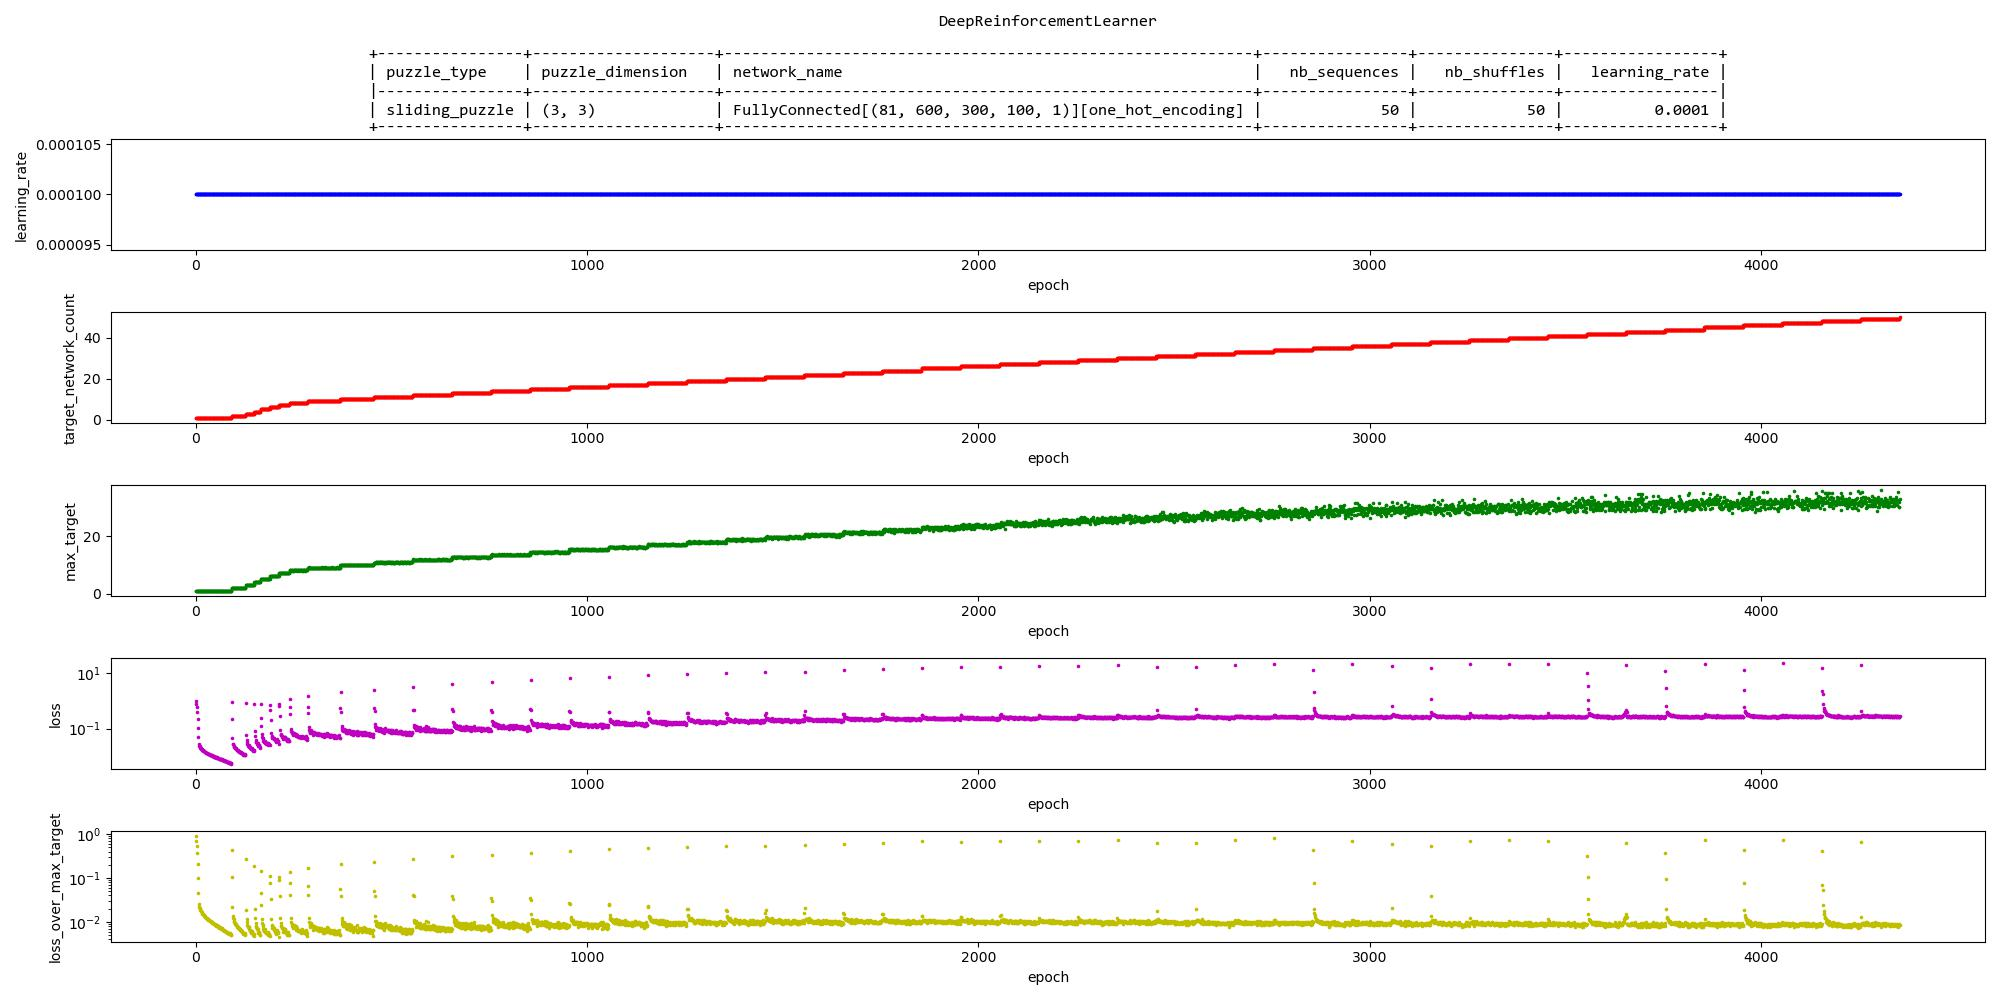
\includegraphics[align=c, scale=0.42]{./Figures/33SPDeepReinforcementLearning}
\caption[33SPDeepReinforcementLearning]{\textbf{DRL} of the 3x3 \textbf{SP}}
\label{fig:33SPDeepReinforcementLearning}
\end{figure}

Notice that the DeepLearner and DeepQLearner have very similar sets of parameters and track similar metrics during their learning for later display, but I shall not detail it here since there is not much extra insight to be had compared to the DeepReinforcementLearning example we just went through.





\Subsection{Solvers' comparison}

\begin{figure}[H]
\centering
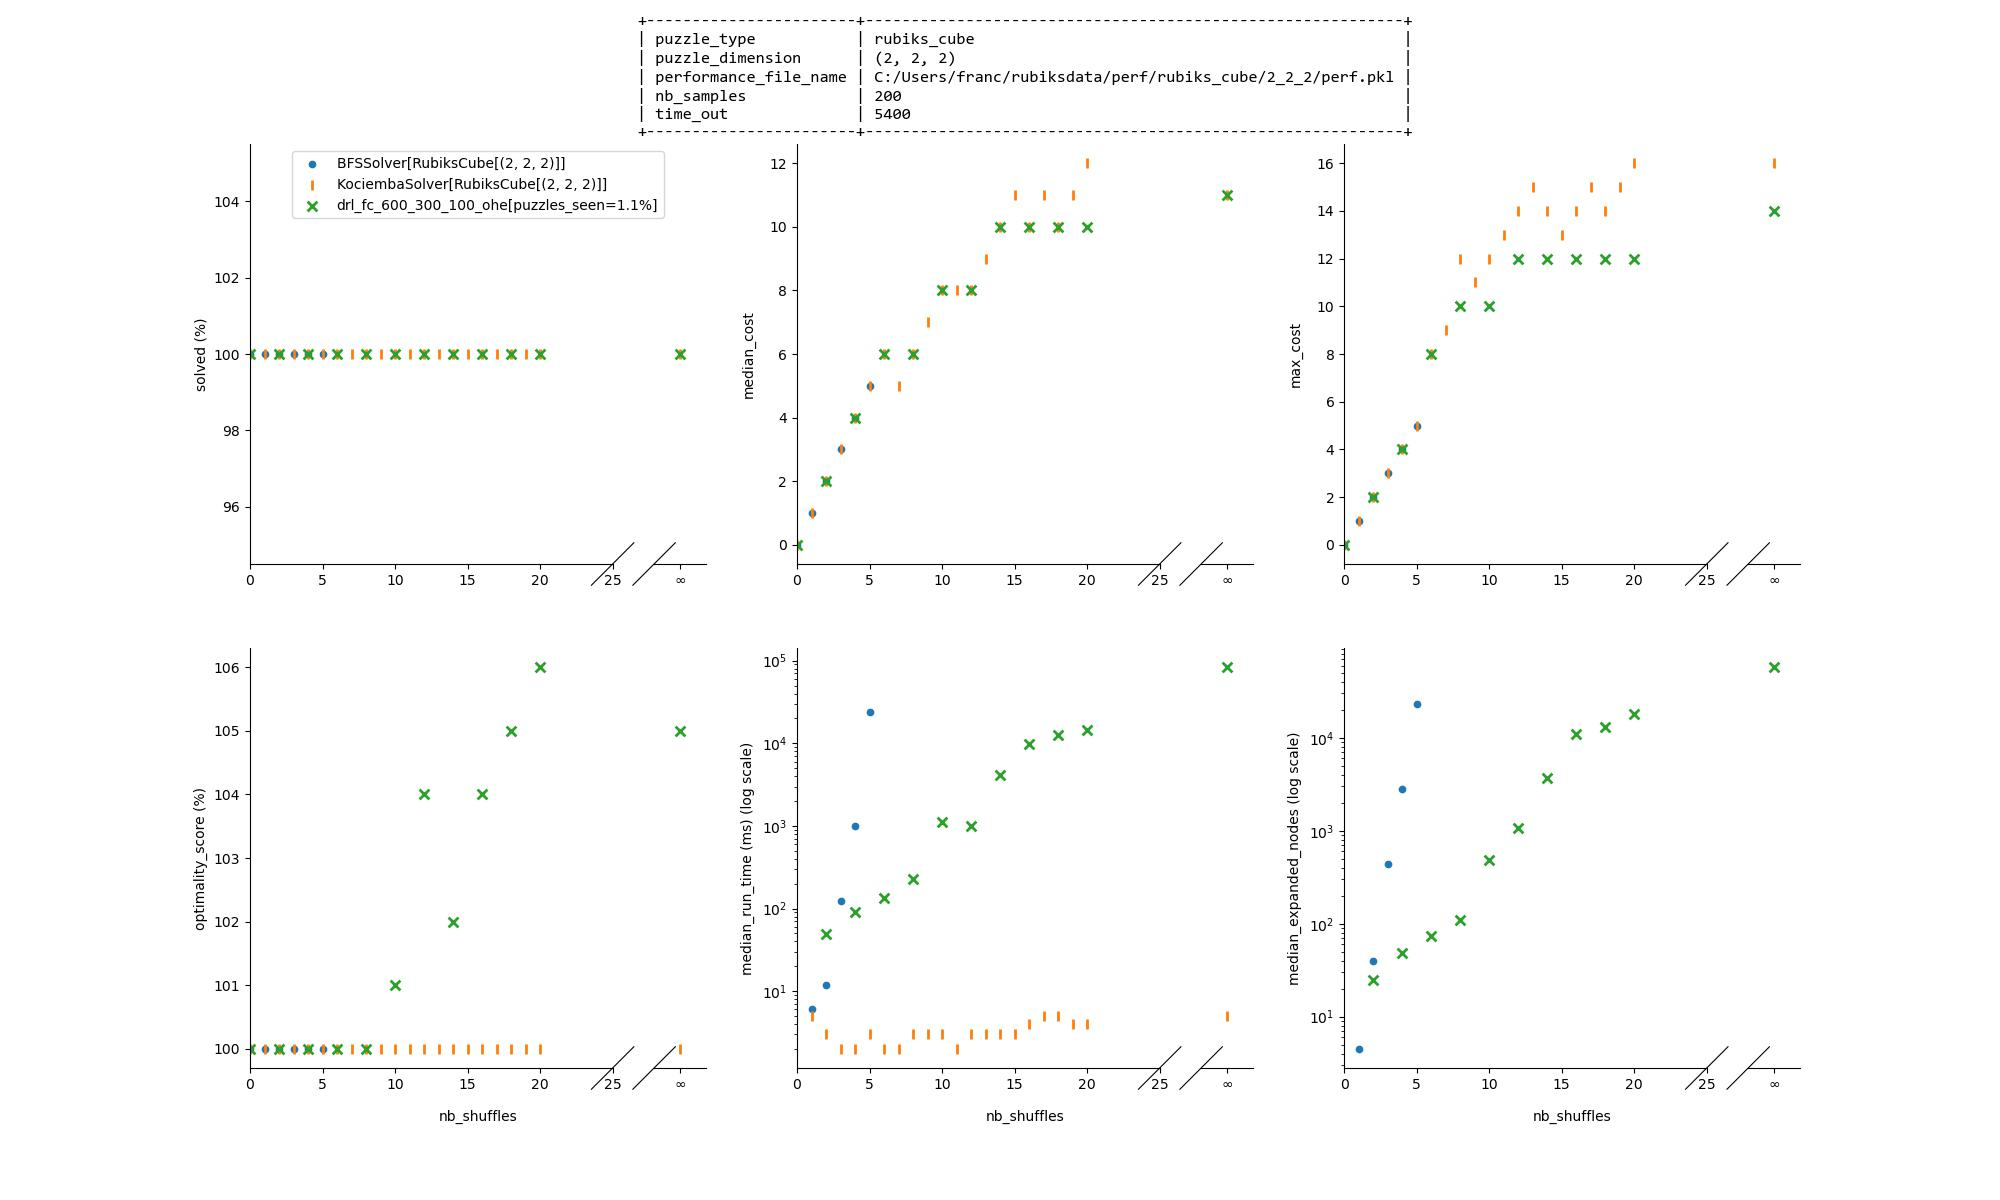
\includegraphics[scale=0.60]{./Figures/222RCPerformance}
%\decoRule
\caption[222RCPerformance]{Solvers' performance comparison 2x2x2 \textbf{RC}}
\label{fig:222RCPerformance}
\end{figure}



%-----------------------------------
%	SUBSECTION 1
%-----------------------------------
\Section{3x3x3}
\label{sec:ResRubiks333}

For now just showing Kociemba as a baseline. Will first try out DL trained on data generated from Kociemba, then will try out DRL. If unsuccessful or too slow, might try similar to paper using DQL/MC search.
\\
Notice Kociemba 3, unlike the 2x2x2 implementation that I found on github, does not do automatic color mapping. So if you present it with a cube which is not with the \textit{standard} centers (facing red and white up), it will actually not solve the cube. I have therefore added a bit of logic in Kociemba solver to look for the equivalent cube among the 24 equivalent cubes to the one being solved, with standard colors. We then solve this one using Kociemba and add the whole cube rotations to the solution (which in my code are deemed to have 0 cost anyway). This way, not only can I use Kociemba 3 to solve any (solvable) 3x3x3 cube irrespective of rotations, but I can also use that in A* or to train a DL network (also for A*)




\begin{figure}[H]
\centering
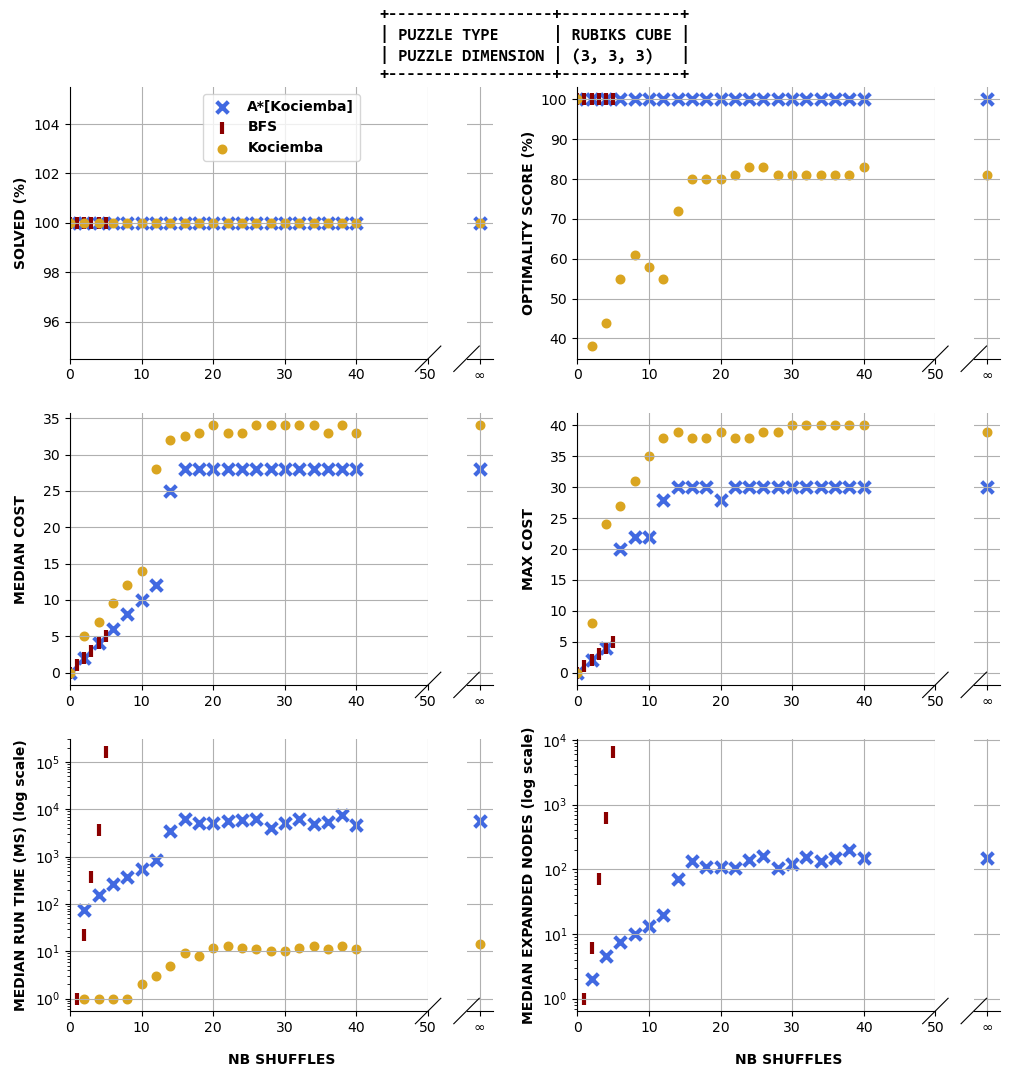
\includegraphics[scale=0.50]{./Figures/333RCPerformance}
%\decoRule
\caption[333RCPerformance]{Solvers' performance comparison 3x3x3 \textbf{RC}}
\label{fig:333RCPerformance}
\end{figure}
